%
% File acl-hlt2011.tex
%
% Contact: gdzhou@suda.edu.cn
%%
%% Based on the style files for ACL2008 by Joakim Nivre and Noah Smith
%% and that of ACL2010 by Jing-Shin Chang and Philipp Koehn


%\documentclass{article}  
\documentclass[12pt]{IEEEtran}

\renewcommand{\baselinestretch}{1.2} 

\usepackage{multirow, rotating, amsmath, wasysym}
\usepackage[tight]{subfigure} 
\usepackage[ruled,linesnumbered,vlined]{algorithm2e} 
\usepackage{hyperref}

\usepackage{color,soul}
\usepackage{listings}
\usepackage{array, graphicx}
\usepackage{subfigure}
\usepackage{caption} 

\graphicspath{{../}{figures/}}


\mathchardef\Gamma="0100 \mathchardef\Delta="0101
\mathchardef\Theta="0102 \mathchardef\Lambda="0103
\mathchardef\Xi="0104 \mathchardef\Pi="0105
\mathchardef\Sigma="0106 \mathchardef\Upsilon="0107
\mathchardef\Phi="0108 \mathchardef\Psi="0109
\mathchardef\Omega="010A

\newcommand{\ovspace}[1]{\vspace{#1}}

\newcommand{\outline}[1]{}%{\textbf{#1}}

\newcommand{\dl}{\mbox{$\, [ \hspace*{-1.5pt} [\,$}}
\newcommand{\dr}{\mbox{$\, ] \hspace*{-1.5pt} ]\:$}}
\newcommand{\da}{\mbox{$\, A \hspace*{-6.75pt} A \,$}}
%\newcommand{\drightarrow}{\mbox{$\rightarrow \hspace*{-8pt} \rightarrow$}}

\newcommand{\BA}{\mbox{${\bm{a}}$}}
%\newcommand{\BB}{\mbox{${\bm{c}}$}}
\newcommand{\BC}{\mbox{${\bm{c}}$}}
\newcommand{\BD}{\mbox{${\bm{d}}$}}
\newcommand{\BE}{\mbox{${\bm{e}}$}}
\newcommand{\BO}{\mbox{${\bm{o}}$}}
\newcommand{\BP}{\mbox{${\bm{p}}$}}
\newcommand{\BQ}{\mbox{${\bm{q}}$}}
\newcommand{\BR}{\mbox{${\bm{r}}$}}
\newcommand{\BV}{\mbox{${\bm{v}}$}}
\newcommand{\BL}{\mbox{${\bm{l}}$}}
\newcommand{\BI}{\mbox{${\bm{i}}$}}
\newcommand{\BH}{\mbox{${\bm{h}}$}}
\newcommand{\BS}{\mbox{${\bm{s}}$}}
\newcommand{\BB}{\mbox{${\bm{k}}$}}

\newcommand{\wrapbox}[1]{\framebox{\begin{tabular}{c}#1\end{tabular}}}
\newcommand{\CodeIn}[1]{{\small\texttt{#1}}}
\newcommand{\Section}[1]{Section~\ref{sec:#1}}
\newcommand{\SFigure}[2]{Figure~\ref{fig:#1}(#2)}

\usepackage{cite}
\usepackage{xspace}
\usepackage{url}
\usepackage{graphicx}
\usepackage{latexsym}
\usepackage{amssymb}
\usepackage{amsfonts}
%\usepackage{times}
\usepackage{psfrag}
%\usepackage{subfigure}
\usepackage{wrapfig}
\usepackage{comment}
%packages for algorithms
%\usepackage{algorithm}
%\usepackage{algorithmic}
\usepackage{alltt}
\usepackage{color}

\newtheorem{defn}{Definition}[section]
\newtheorem{exmp}{Example}[section]
\newtheorem{thrm}{Theorem}[section]
\newtheorem{prop}{Proposition}[section]
\newtheorem{lemm}{Lemma}[section]
\newtheorem{obsv}{Observation}[section]
\newtheorem{corr}{Corollary}[section]

%\addtolength{\textheight}{.23in} \addtolength{\textwidth}{.15in}
%\addtolength{\topmargin}{-.23in}
%\addtolength{\oddsidemargin}{.1in}
%\addtolength{\evensidemargin}{.1in}

\newtheorem{thm}{Theorem}
\newtheorem{dfn}{Definition}
\newtheorem{lem}{Lemma}
\newtheorem{cor}{Corollary}
\newcommand{\ie}{\emph{i.e.}\xspace}
\newcommand{\eg}{\emph{e.g.}\xspace}
\newcommand{\etc}{\emph{etc.}\xspace}
\newcommand{\etal}{\frenchspacing{}\emph{et al{.}}\xspace}
%\newcommand{\etal}[1]{{\sl et al.{#1}}}

%\newcommand{\thm}[1]{Theorem~\ref{thm:#1}}
%\newcommand{\lem}[1]{Lemma~\ref{lemma:#1}}
%\newcommand{cor}[1]{Corollary~\ref{cor:#1}}
\newcommand{\fac}[1]{Fact~\ref{fact:#1}}
\newcommand{\Table}[1]{Table~\ref{tab:#1}}
\newcommand{\Figure}[1]{Figure~\ref{fig:#1}}

%\theoremstyle{plain}
\newtheorem{property}{Property}[section]
\newtheorem{lemma}{Lemma}[section]
\newtheorem{corollary}{Corollary}[section]
\newtheorem{theorem}{Theorem}[section]

%\theoremstyle{definition}
\newtheorem{notation}{Notation}
\newtheorem{Definition}{Definition}[section]

%\theoremstyle{remark}
\newtheorem{fact}{Fact}[section]
\newtheorem{observation}{Observation}[section]
\newtheorem{insight}{Insight}[section]

%%\algorithmstyle{definition}
%\algsetup{indent=1em}
%\renewcommand{\algorithmicrequire}{\textbf{Input:  }}
%\renewcommand{\algorithmicensure}{\textbf{Output:}}
\newcommand{\factorial}{\ensuremath{\mbox{\sc Factorial}}}

\newcommand{\Comment}[1]{}

\renewcommand\floatpagefraction{0.999}
\renewcommand\topfraction{0.999}
\renewcommand\bottomfraction{0.999}
\renewcommand\textfraction{0.001}
\setcounter{totalnumber}{5}
 
\newcommand{\subfigs}{\hspace{-0.10in}}  
 
\author{
\begin{tabular}[t]{c@{\extracolsep{8em}}c} 
Nan Xia  & Zhuangdi Zhu \\
Michigan State University & Michigan State University \\ 
nanxia@msu.edu & zhuzhuan@msu.edu
\end{tabular}
}


\title{Deep Tweeting:\\ 
Twitter Sentiment Analysis using Recursive Deep Models}




\begin{document}
\maketitle


\sloppy{
% !TEX root = /Users/zhuzhuangdi/Desktop/MSUCourses/NaturalLanguageProcessing842/CSE842/FinalReport/latex/final.tex

\begin{abstract}
In this project, we explore the application of Recursive Neural Network (RNN) models on the sentiment analysis task with Twitter.
%
Twitter is a dominating social media that allows users to post 140-character long micro blogs called tweets, which usually convey large amount of information that can be further used for opinion mining on important social events. 
%
Different from prior work using bag-of-words models, we plan to evaluate how deep learning models can be used to improve the accuracy of sentence-level sentiment analysis in micro-blogging domain. 
%
We use word-to-vector approaches to map each word in a tweet into a vector representation which capture the semantic relevance among different words, and use the vector representation as inputs to training our RNN classifier.
%
Our RNN approach outperforms traditional bag-of-words based classifiers by over 20\% percent accuracy.
%
It also outperforms a Convolution Neural Network based approach by over \% percent accuracy, with a faster convergence rate.
%
Our model can also be scaled to solving multi-class classification problems.

% We semantically compose vector-space representations for tweets to capture their parse structure.
%Especially, we will use the treebank provided by Stanford to generate a parse tree for each tweet, and use it as the input to the RNN model. 
%

%

\end{abstract}
%\keywords{Semantic Analysis; Twitter; Micro-blogging; Parse Tree;  Deep Learning } 
\vspace{0.1in}
% !TEX root = /Users/zhuzhuangdi/Desktop/MSUCourses/NaturalLanguageProcessing842/CSE842/FinalReport/latex/final.tex

\section{Introduction}
\subsection{Motivation}
%In this project, we will address the problem of sentence-level sentiment analysis.
%
In this project, we will propose and implement deep learning models to conduct text sentiment analysis.
%
Especially, we will use Recurrent Neural Network models to classify sentiment labels of tweets, and see how deep learning models can improve the classification accuracy, compared with bag-of-words methods such Naive Bayes or Support Vector Machine. 
%
Twitter is a popular microblogging platform that allow users to post 140-character-constrained microblogs called tweets, which reveal large amount of information about public opinion in real time \cite{pak2010twitter}. 
%
The results of sentiment analysis on twitter can be further used for opinion mining in many socio - economical phenomena.
%, including social, cultural, political or financial areas. 
Prior work has applied twitter sentiment analysis into areas such as president-election prediction \cite{tumasjan2010predicting,wang2012system}, market targetting\cite{bollen2011modeling}, and stock price estimation\cite{bollen2011twitter}.
% 
It is  a meaningful research area that will continue to attract interests and efforts from academia.

\subsection{Background}
The explosion of data about public opinion on social networks and review websites in recent years leads to an ever-growing demand in opinion mining in many soci-economical areas.
%
This demand can be satisfied by sentiment analysis, a popular NLP technique that relies on large amount of data labeled with sentiment categories.
% 
With the easily achievable online data that reveal user sentiments, the potential of sentiment analysis has been exploited in various areas, such as high frequency trading, election prediction, and stock price estimation.

A basic method of sentiment analysis is to use bag-of-words based model.
%
This kind of models ignore the order of words in a context, and the predicted label is dominated by a few words with strong sentiment.
%
The most frequently studied model based on bag-of-word features is Naive Bayes, which is a probabilistic classifier.
%
The rationale behind Naive Bayes model is that given a document, it will generate the class label that has the maximum posteriror probability given the document.
%
This model was first applied to text classification by Mosteller and Wallace in 1964 \cite{mosteller1964inference}.
%
Bag-of-words based models work well in document-level analysis.
%
However, for short reviews or comments in one sentence, the classification accuracy of this model is around 80\%\cite{wang2012system}.
%
Since the dominant type of data online is usually short comments or reviews, there is a need to better predict sentiment in a sentence-level. 

Another kind of methods is to is to use deep learning approaches.
%
With the blossom of large amount of corpus available on the internet, deep learning approaches using neural networks have earned increasing popularity the filed of Natural Language Processing.
%
Researchers from Stanford University have proposed complex neural network models  to conduct sentence-level sentiment analysis.
%
 An example is the Matrix-Vector Recursive Neural Network (MV-RNN), proposed by Socher \etal \cite{socher2012semantic}.
%
This kind of models takes input a parse tree of a sentence, and generates the sentiment category of the root node of the parse tree by recursively building it in a bottom-up fasion.
%
They work well only for sentences follow correct gramma or syntactic rules, but are not suitable for tweets, which have informal expression both in gramma and in lexicon.
% 




% !TEX root = /Users/zhuzhuangdi/Desktop/MSUCourses/NaturalLanguageProcessing842/CSE842/FinalReport/latex/final.tex

\section{Related Work}  
%
There are several previous researches on NLP techniques designed for Twitter data. Hereby are some most relevant work for our reference:

Kouloumpis \etal conducted sentiment analysis on twitter data, and their focus is to evaluate the effects of different kinds of features on the classification accuracy\cite{kouloumpis2011twitter}.
%
They explored the features of n-gram, POS, and especially, micro-blog features such as emotions and hastags.
%
Their findings are that POS features not be useful for twitter sentiment analysis, while micro-blog features are best indicators of sentiment labels.
%
Their best performance is 0.75 on average accuracy.

Apoorv \etal  proposed a tree-kernel based model to do sentiment analysis\cite{agarwal2011sentiment}. 
%
They designed a new tree representation for tweets as inputs to the kernel to obviate the need of extracting features.
%
The best performance of their model is 60.83\% accuracy.

Wang \etal use a naive Bayes model to  conduct twitter sentiment analysis in order to analyze the president election cycle\cite{wang2012system}.
%
They adopted unigram features as the classifier input.
%
The key novelty of this work is that they implemented an analysis system that takes real-time twitter messages as inputs, instead of doing post-facto analysis.
%
Their discovery is that tweet volume is largely driven by campaign events.

Go \etal use distant supervision to conduct Twitter sentiment classification \cite{go2009twitter}.
%
The key novelty of their work is the use of emotion features for distant supervised learning.
%
They explored with different classifiers, such asNaive Bayes, Maximum Entropy, and SVM, with a best performance of around 80\%  for  average accuracy.
 
More neural network-based sentiment analysis models have been proposed recently.
%
Kim \etal used a standard Convolution Neural Networks to classify tweets, with a best performance of 89.6\%
% 
Socher \etal created a recursive model to build the sentiment label of a sentence through its parse tree \cite{socher2012semantic}. 
%
Each constituent in the sentence is associated with a vector-matrix representation.The vector conveys the meaning of the constituent, while the matrix conveys how it changes the meaning of neighboring constituents.

 
% !TEX root = /Users/zhuzhuangdi/Desktop/MSUCourses/NaturalLanguageProcessing842/CSE842/FinalReport/latex/final.tex

\section{DeepTweeting Sentiment Analysis System} 
We implement a system that utilizes a recursive a Recurrent Neural Network (RNN) model to predict the sentiment classes of different tweets.
%
Especially, we use a specialized RNN named Long Short Term Memory (LSTM) network as our system model.
%
We adopt two pre-processing steps to map each tweet into a three-dimensional matrix representation, so that the relevant meaning among different words in the Twitter corpus can be captured.
%
The output of our model is a probability distribution of all the sentiment labels for a tweet.
%
In our project, we only consider two-class sentiment classifications, that is, a tweet can be either negative or positive.
%
However, our model can be easily scaled to multi-sentiment classification problems. Our system overview is shown in Figure \ref{fig:systemoverview}.

\begin{figure}[htb]
	\centering
	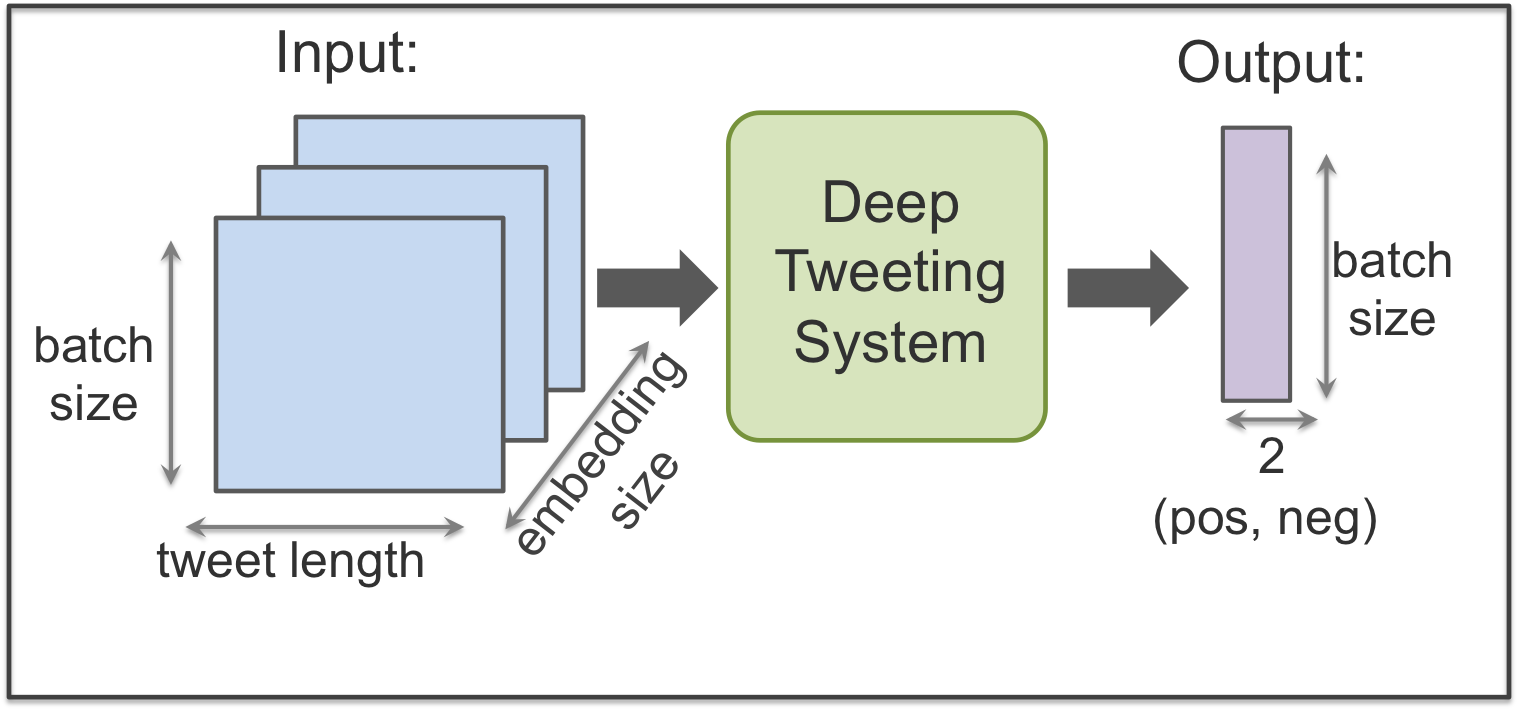
\includegraphics[width=0.9\linewidth]{DeepTweetingOverview}
	\caption{Sentiment Analysis System Overview}
	\label{fig:systemoverview}
\end{figure}


% based on the vector-space representation of the tweet.
%The intuition is that: for sentence-level messages like tweets, the meaning of this expression should be derived based on the meanings of its words and the rules used to combine them.
%We will semantic compositionnality of tweets, and generate a parse tree for each tweet as the input of this model.  
%
%the Stanford Parser\cite{klein2003accurate} to for parse tree generation.
%

%proposed by \cite{kouloumpis2011twitter} %
%Moreover, we  also plan to explore the possibility to use hashtags and emotions as feature to improve the sentiment classification accuracy of our model.
%
%of pairs of words whereas we would like nonlinear functions to compute compositional meaning representations for multi-word phrases or full sentences.
%
%For evaluation, we plan to use two baselines to compare with our approach: a Naive-Bayesian model using bi-grams as features, and an SVM model using Term frequency ITF-IDF as features.
%
%%As a special task for sentence-level sentiment analysis, twitter sentiment analysis 
%The features of informal language, the frequent use of emotions and hashtags, as well as the lengths constraints of tweets make the analysis of twitter 




%It's an open question how well the features and techniques used on more well-formed data will transfer to the microblogging domain.
%Many researchers, such as Mullen and Collier \cite{mullen2004sentiment}, have used empirical distributions of words and hand-selected features to perform this analysis with a variety of standard machine learning models, such as SVMs and Naive-Bayes.
%These approaches have been effective on certain datasets, but have poor cross-domain performance and require significant domain-specific tailoring. 
%
%These prove to be a weak point in many models. 
%Therefore, we can take from this that explicit modeling of these more complicated linguistic effects can be beneficial to any sort of semantic analysis - in particular, including sentiment analysis. 
%%
%%Additionally, the datasets these models are based upon generally only contain sentiment labels for the entire sentence, making it ambiguous which part of the sentence was responsible for the sentiment.
%The very nature of the microblogging domain make Twitter sentiment analysis a very special task in sentence-level sentiment classification task.
 
\subsection{Preprocessing}
We use word embedding to map Chinese characters from the poem corpus to vectors of real numbers, which consists of two steps: tokenization and word embedding.
% 
%Especially, we consider both semantic and rhythmic relevance in the word-to-vector transformation.
%
\subsubsection {Tweet Tokenization}
%We associated each Chinese character with a unique value as its ID, so that the most frequent word in the corpus  will get a highest value, while the less frequent words have smaller ones.
%During our project, we carefully tune the size of the vocabulary set $|V|$ so that the most $|V|$ frequent words will be kept in our vocabulary, while the other unfrequent words will be mapped to the same \emph{UNKOWN} token to avoid overfitting.
%
Then we use the ID as the feature for each word to train our word embedding matrix.
%Each character has a unique index ID, while characters share the same simple or compound vowels will have the same rhyme ID. 
%For example, in Figure \ref{fig:rhyme_features}, the two Chinese characters, \emph{guang} and \emph{shuang}, will maintain the same rhyme ID.
%The rhymes can be extracted using a python module called \emph{pinyin}.
%
As a specialized corpus, tweet data contain large amount of micro-blogging features, such as emojis, hand-shorts, hashtags and user mentions \cite{kouloumpis2011twitter}.
%
A straight-forward approach to preprocess these data is to consider all above features as noises and remove them from each tweet.
%
However, this may lead to information loss, as this micro-blogging features usually reveal strong sentiment trends.
%
So our approach is to map each kind of above-mentioned feature into a specific keyword using regular expression:
\begin{itemize}
\item Emotions: We map all different kinds of emotions in a tweet to the same keyword ${<emoji>}$.
\item Shorthands: We collect most popular shorthands in twitter. For each tweet, we convert the shorthands in it into a phrase revealing its sentimental tendency. For example, \emph{3$>$} means \emph{love}.
\item Hashtags: We seperate the hashtag from its following word, and map the hashtag to a keyword \emph{hashtag}. For example, $\# amazing$ will be $<hashtag>$ $amazing$.
\item Mentions: we map all user mentions to a keyword ${<user>}$. 
\item Duplications: For each word in a tweet, if there are duplicate letters for more than three times, such as \emph{cooooooool}, we will only keep two letters of them, so the above-mentioned word will change to \emph{cool}.
\item URLs: Since URLs are usually irrelevant with the sentiment tendency of the tweet, so we just replace all URLs in tweets with a keyword $<URL>$.
\end{itemize} 


\begin{figure}[ht]
% \hspace{-0.2in}
\begin{minipage}[t]{1\linewidth}
\centering 
\subfigure[]{
   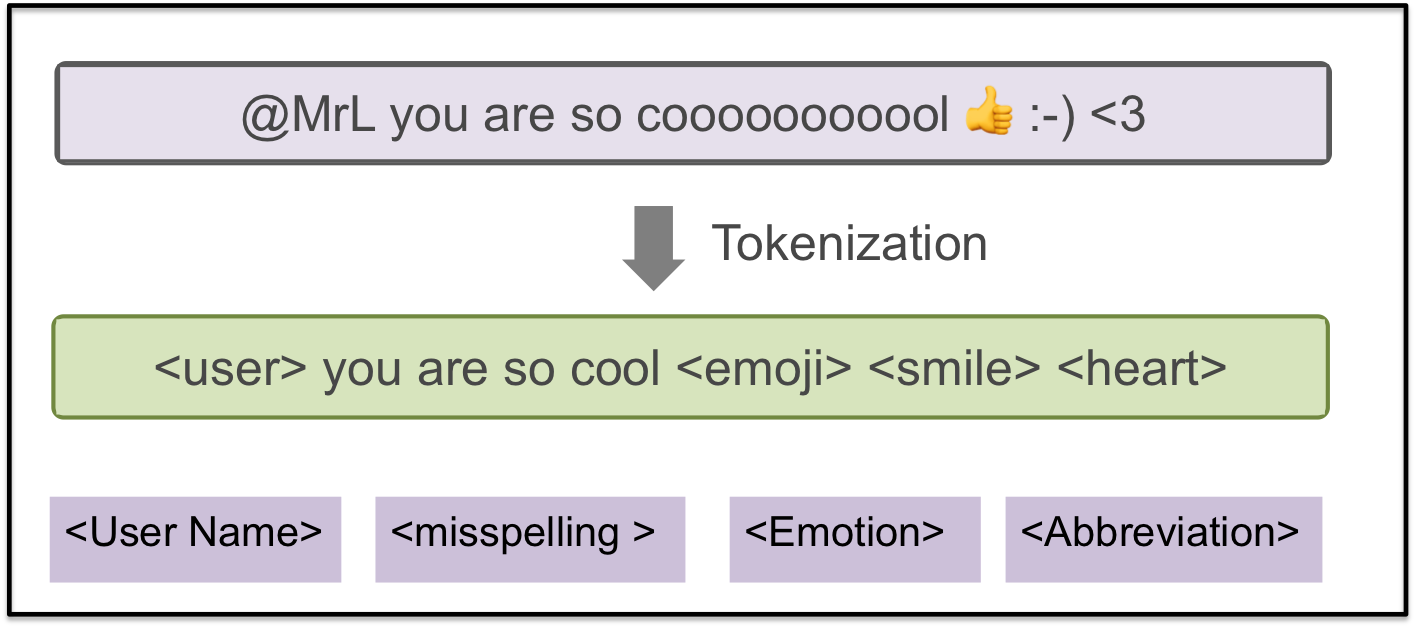
\includegraphics[width=0.9\linewidth] {token1}
   \label{fig:token1}
 } 
% \hspace{-0.2in}
 \subfigure[]{
   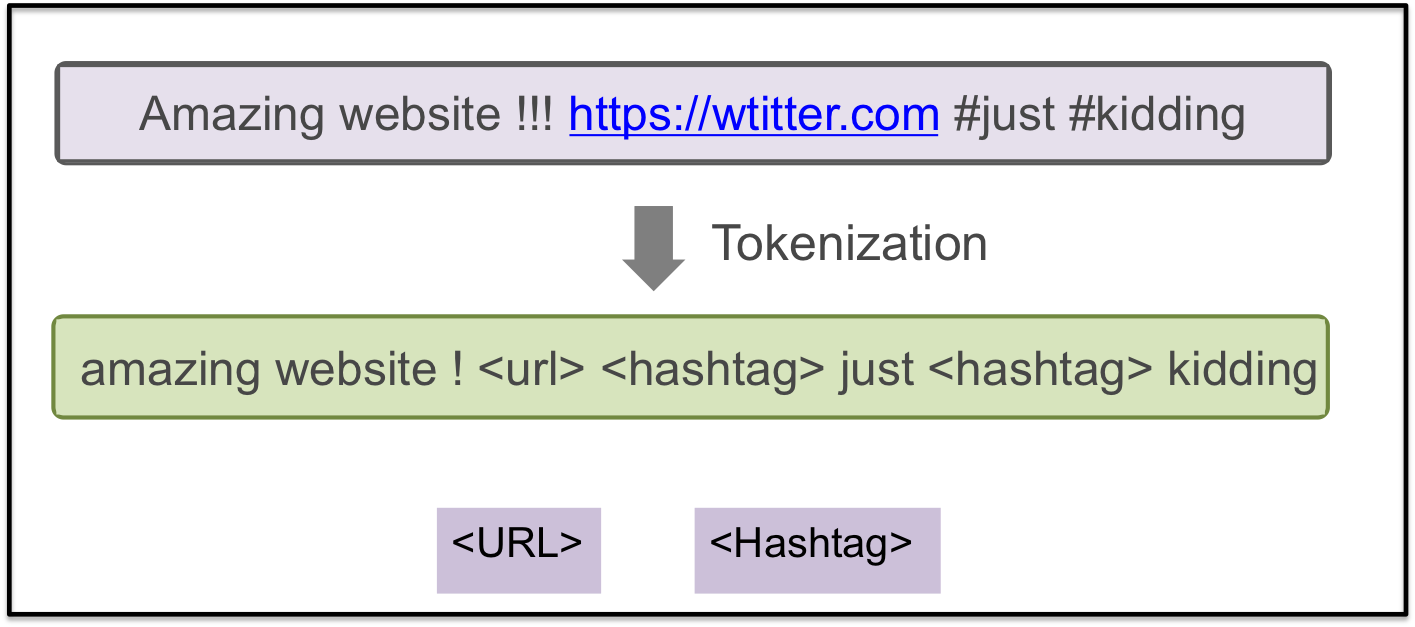
\includegraphics[width=0.9\linewidth] {token2}
   \label{fig:token2}
 } 
\caption{\textbf{Twitter Tokenization with respect to different micro-blogging features}}
\label{fig:token}
\end{minipage}
\end{figure}


\subsubsection {Word to Vector Representation}
We cannot feed our RNN model with raw tweet text, so a vector representation for tweet is necessary.
%
Especially, we adopt a skip-gram model to get a word-embedding matrix for all words in the Twitter corpus\cite{mikolov2013efficient}, so that the semantic relevance  among different words can be captured and used as inputs to the RNN model.
%
We get this matrix by training a single-layer neural network. 
%and the parameter matrix inside the network will be our word embedding matrix.
%
 The input of the model is a single word $w_I$, and the output is the words in its context $\{w_{O,1},w_{O,2}, \dots, w_{O,C}\}$ defined by a word window of size $C$.
%
As shown in Figure \ref{fig:skip_gram},  $x$ represents the one-hot encoded vector corresponding to the
input word in the training text,
%
 and $\{y_1, y_2, \dots, y_C\}$ are the one-hot encoded vectors corresponding to the output words in the training text.
 %
 The $V \times N$ matrix $W$ is the weight matrix between the input layer and hidden layer whose
$i^{th}$ row represents the weights corresponding to the $i^{th}$ word in the vocabulary. 
%
This weight matrix is what we call the word-embedding matrix because it contains the
vector encodings of all of the words in our vocabulary.
%
We can use this word-embedding matrix to capture the semantic relevance among words, so that two words with close semantic meanings will have smaller distance in the vector space.

\begin{figure}[htb]
	\centering
	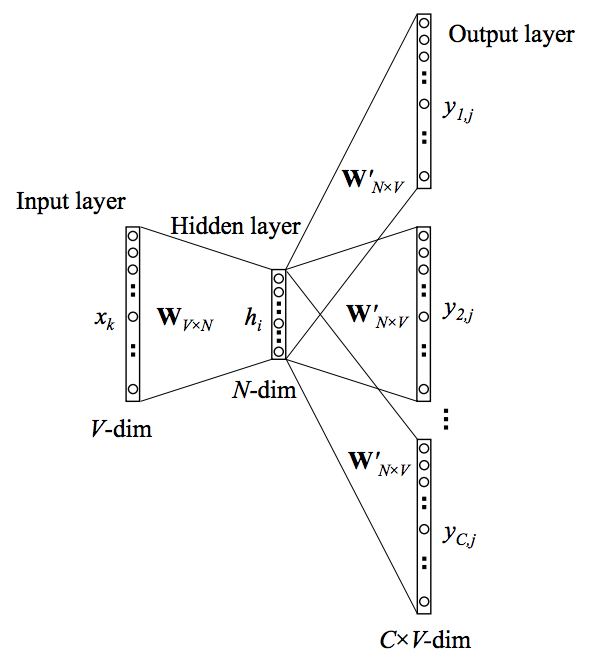
\includegraphics[width=0.9\linewidth]{skip_gram}
	\caption{A skip gram neural network}
	\label{fig:skip_gram}
\end{figure} 

\begin{figure}[htb]
	\centering
	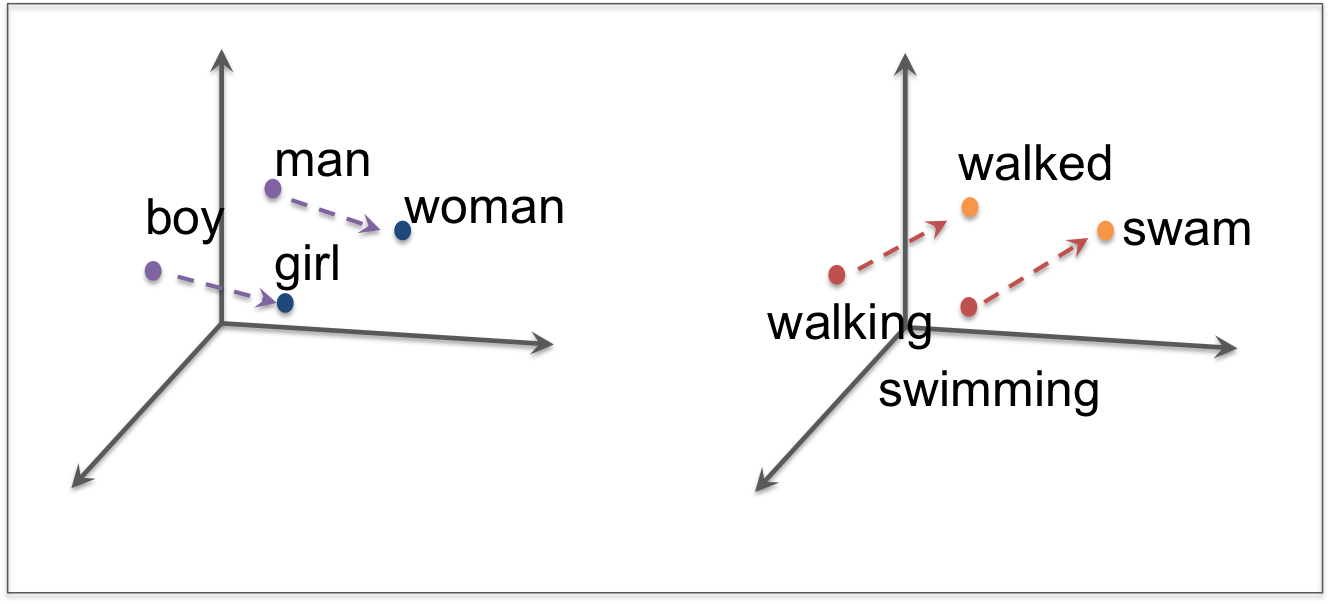
\includegraphics[width=0.9\linewidth]{word2vec}
	\caption{Vector Representation of words}
	\label{fig:word2vec}
\end{figure}


\subsection{Recurrent Neural Network}  
Recurrent Neural Networks (RNN)s are a specialized neural network that consists of multiple copies of the same network cell, as shown in Figure \ref{rnn_overview}.
%
Due to this recursive structure, it is suitable for processing sequential data  \cite{rumelhart1986}.
%
%It is specialized for processing a sequence of valuesx $x^{(1)}, x^{(2)}, \dots, x^{(t)}$.
%
For each network cell $A_t$ in the RNN model, its has an input $s_t$, a hidden state $s_t$, and generates an output $h_t$.
%
The output and hidden state are then scaled and feed as inputs to its successor network cell.
%Parameter sharing across the different parts of the model is the key idea that makes RNNs to be able to deal with the sequential data.
%
However, a simple RNNs cannot learn long time dependency, because during the optimization step, the parameter matrix this term tends to vanish or explode very fast due stochastic gradient \cite{goodfellow2016deeplearning}.
%
To solve this challenge, specialized RNNs with gates is proposed and becomes one of the most effective practical models that used for sequential data.
\begin{figure}[htbp]
	\centering
	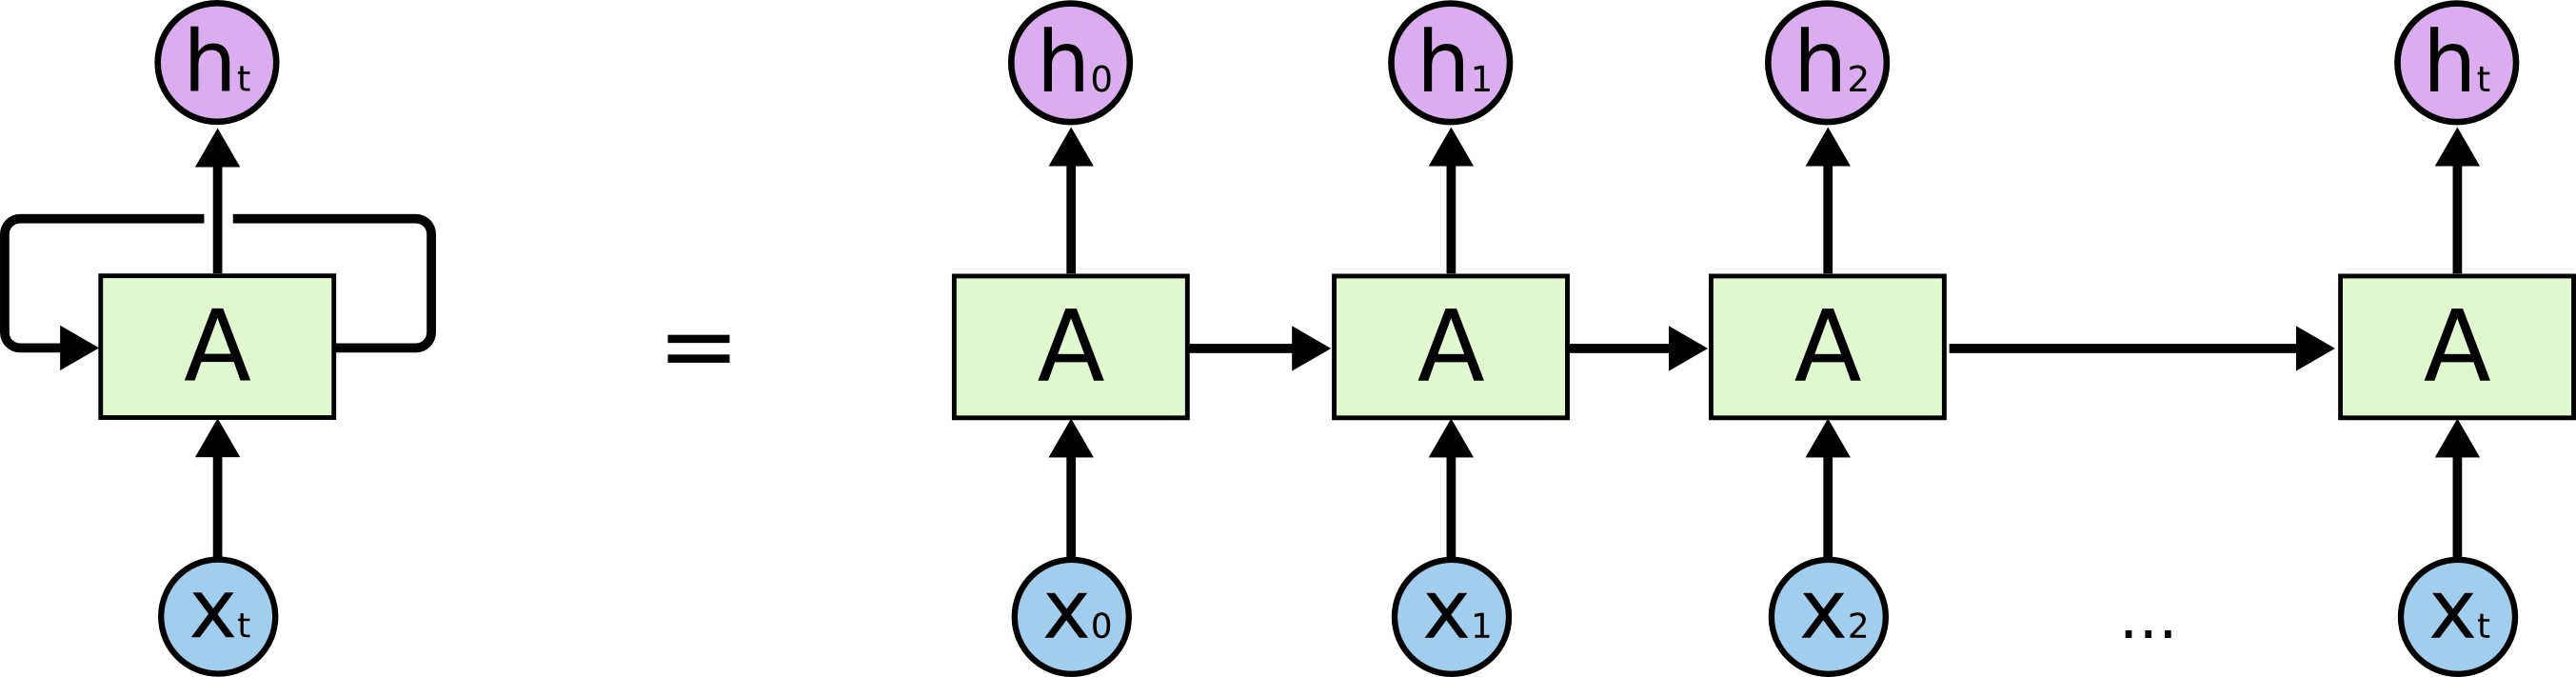
\includegraphics[width=0.9\linewidth]{rnn_overview}
	\caption{A Recurrent Neural Network}
	\label{fig:rnn_overview}
\end{figure}




\subsubsection{Long Short Term Memory}
In our project, we will use a specialized RNN network called Long Short Term Memory (LSTM).
%
Long Short Term memory (LSTM) network is a branch of gated RNNs that can capture long term dependencies when processing sequences of input texts..
%
It is widely used in various machine learning and NLP applications, such as speech recognition, machine translation, and handwriting generation\cite{hochreiter1997lstm} .
%
Gates are a way to optionally let information through. They are composed out of a sigmoid neural net layer and a pointwise multiplication operation. 
%
A LSTM network contains recursive LSTM network cells, each of which consists of the following gates:
\begin {itemize}
\item {Forget gate \(f_i\):} 
\[ f_t =  \sigma (W_f \dot [h_{t-1} , x_t] + b_f ) \]
%\[f_i^{(t)} = \sigma (b_i^f + \sum_{j}U_{i,j}^f x_j^{(t)} +\sum_{j}W_{i,j}^f h_j^{(t-1)} ) \].
%
It generates a scale parameter between 0 and 1 for each component in the previous LSTM cell $C_{t-1}$, based on the current input $x_t$ and previous output \( h_{t-1} \).
%
%Where \(\boldsymbol{x}^{(t)}\) is the current input vector and \(\boldsymbol{h}^{(t)}\) is the current hidden layer vector, containing the outputs of all the LSTM cells. \(\boldsymbol{b}^f\), \(\boldsymbol{U}^f\), and \(\boldsymbol{W}^f\) are biases, input weights, and recurrent weights of the forget gate, respectively. 

\item {External input gate \(i_t \): } the external input gate unit is computed with the following equation:
\[i_t = \sigma (b_i +  W_i  \dot [h_{t-1}, x_t] ) \]

\item {Update gate \( \tilde{C_t} \):} 
This gate updates the internal state of the LSTM cell by the following equation:
\begin{small}
\[  \tilde{C_t} = \tanh (W_C \dot [h_{t-1}, x_t ] + b_C )  \]
\end{small}

\item {Output gate \(h^{(t)}\) and \(q_i^{(t)}\) :}  The output \(h^{(t)}\)
and the output gate \(q_i^{(t)}\) are updated using sigmoid function also:
\begin{eqnarray*}
o_{(t)} &=& \sigma (W_o [h_{t-1} , x_t ] + b_o ) \\
h{(t)} &=& \tanh (C_t) o_{(t)}
\end{eqnarray*}

\end{itemize}



%The key idea of LSTM is to introduce a self loop so that . 
%As shown in Figure \ref{fig:lstm}, the self loop (internal recurrence) is located in "LSTM cells" with outer recurrence like ordinary recurrent network. The weight of self-loop is controlled by a forget gate 
 
  

Using the above four gates in a LSTM cell,  the gradient can flow for long duration , and therefore LSTM can learn long-term dependencies more effectively than normal RNNs. 

\begin{figure}[htb]
	\centering
	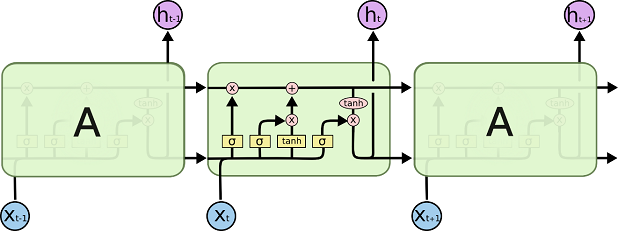
\includegraphics[width=0.9\linewidth]{lstm}
	\caption{A Long Short Term Memory network}
	\label{fig:lstm}
\end{figure} 

\begin{figure}[ht]
% \hspace{-0.2in}
\begin{minipage}[t]{1\linewidth}
\centering 
\subfigure[RNN]{
   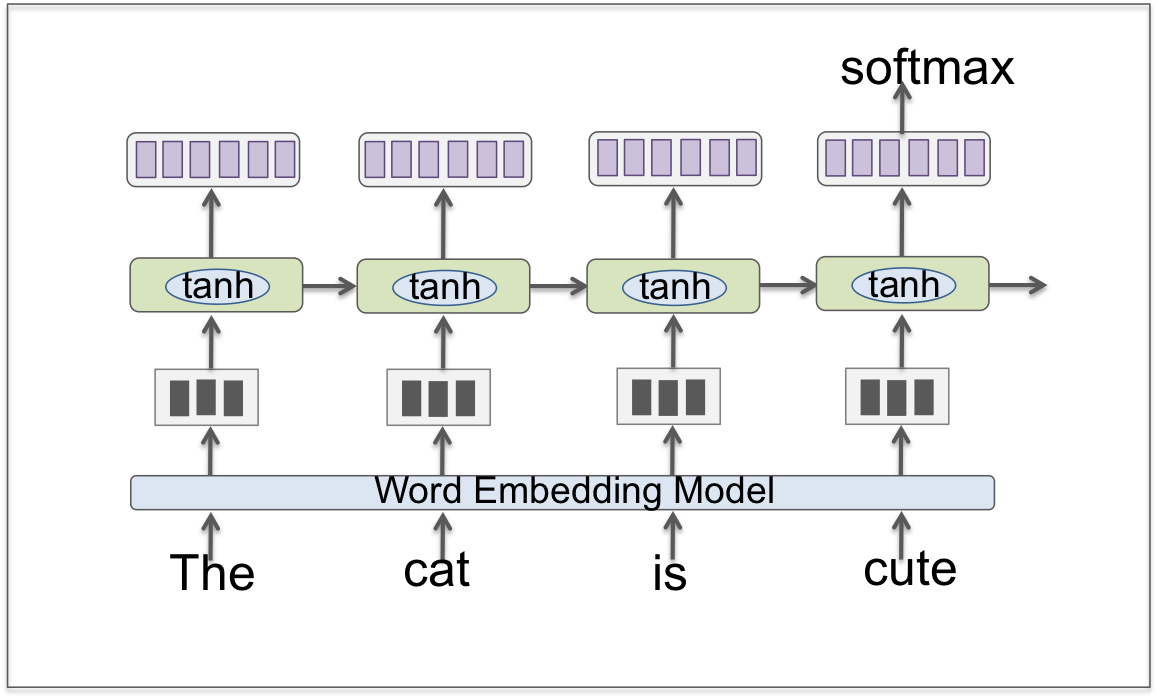
\includegraphics[width=0.9\linewidth] {rnn_workflow}
   \label{fig:rnn_workflow}
 } 
% \hspace{-0.2in}
 \subfigure[LSTM]{
   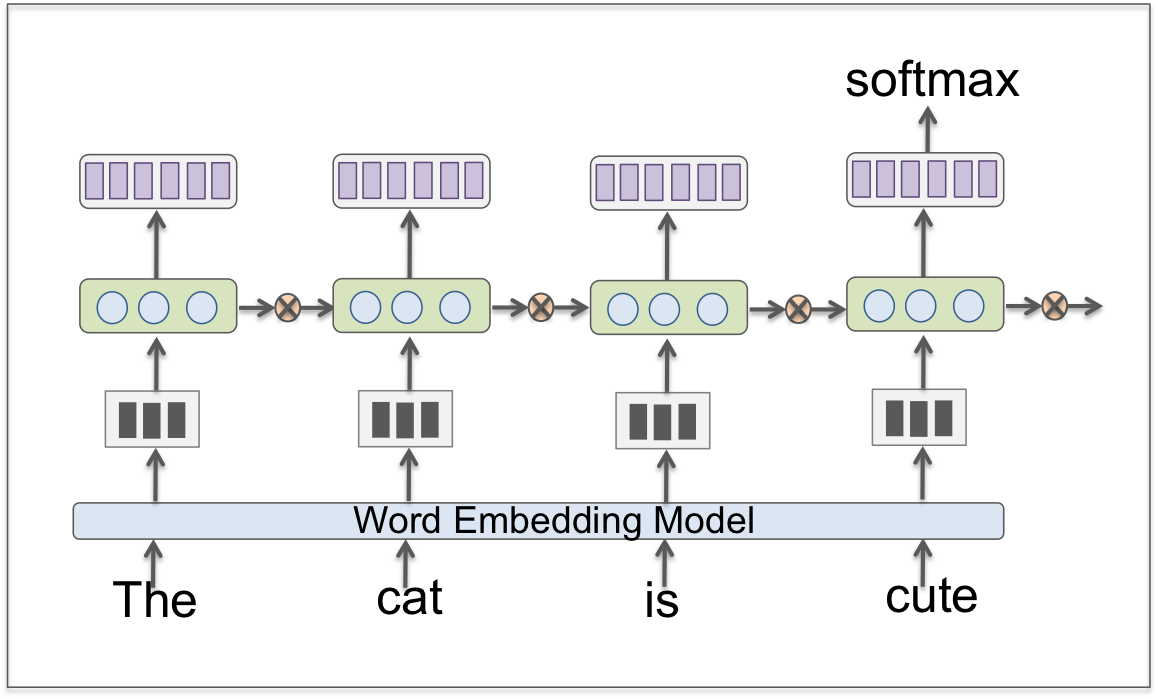
\includegraphics[width=0.9\linewidth] {lstm_workflow}
   \label{fig:lstm_workflow}
 } 
\caption{\textbf{RNN model and LSTM model for sentiment analysis}}
\label{fig:songci}
\end{minipage}
\end{figure}




% !TEX root = /Users/zhuzhuangdi/Desktop/MSUCourses/NaturalLanguageProcessing842/CSE842/FinalReport/latex/final.tex


\section{Evaluation}
We trained and evaluated our sentiment classifier using around 20000 human-labeled tweets, and compare our performance with three baseline sentiment classification approaches.
%
Evaluation shows that our RNN model achieves the highest accuracy compared with baseline models, and has the faster convergence rate compared with models using Convolution Neural Network.
 
\subsection{Available Dataset}\label{subsec:data}
We adopted the Thinknook Dataset\cite{thinknookData} for our evaluation. 
It is composed of tweets from two sources: 
\begin{itemize} 
\item University of Michigan Sentiment Analysis competition on Kaggle\cite{kaggleData}.  
\item Twitter Sentiment Corpus by Niek Sanders\cite{sanderData}.   
\end{itemize} 
%
This dataset contains $1,578,627$ classified tweets since 2012, each row is marked as 1 for positive sentiment and 0 for negative sentiment. 
%
For each sample in the dataset, it contains the tweet ID, the tweet content, and a sentiment label of either \emph{pos} and \emph{neg}. 
%
We extract the tweet content and sentiment labels, and separate the huge dataset into multiple batches of the same size.
%
After preprocessing our data, each batch is a three-dimensional matrix representation which can be used to train and test our RNN model.

\subsection{Baseline Models}
We adopt three baseline approaches to compare with our model: the first two models are based on bag-of-words approaches, that is, these models do not consider the order of words shown in the document, but consider the frequency for a word to appear in the corpus.
\begin{itemize}
\item SVM: For SVM model, we adopt a linear model, and use the Term Frequency - Inverse Document Frequency (TF-IDF) as our input features. TF-IDF is widely used in NLP text classification tasks. It consists of two terms: a term frequency \( tf\) and an inverse document frequency \( idf\):
%\begin{align} 
%tf(t,d) &= 1 + \log(f_{t,d} \\
%idf(t,D) &= log \frac{N}{|\{d \in D: t \in d \}|}
%\end{align}
  
\item Naive Bayes : For naive Bayes model, we use the uni-gram as the input features. Before training model, we adopt the same pre-processing approach as our RNN model.
\item Convolution Neural Network (CNN): We adopt the CNN model for sentiment analysis proposed by Kim \etal \cite{kim2014convolutional}. It applies principals from image processing to a tweet's 2 dimensional sentence vector. In this model, we use a single layer CNN.
\end{itemize}
  


\subsection{ System Implementation} 
%
We used deep learning Python modules called \emph{TensorFlow} \cite{tensorflow} to implement our RNN model. The core parameters are given in Table \ref{fig:rnn_workflow}.
%
The core of the model consists of an LSTM cell that processes one word at a time and computes probabilities of the possible values for the next word in the sentence. 
%
The memory state of the network is initialized with a vector of zeros and gets updated after reading each word. 

\begin{table}[htpb]
\centering
\caption{RNN model parameters}
\label{table:rnn}
\begin{tabular}{|l|l|}
\hline
\textbf{Parameter}      & \textbf{Value} \\ \hline
\textbf{batch\_size}    & 64             \\ \hline
\textbf{embedding size} & 64             \\ \hline
\textbf{hidden layer}   & 50             \\ \hline
\textbf{l2 rate}   & 0.1            \\ \hline 
\textbf{dropout rate}   & 0.5            \\ \hline
\textbf{learning rate}  & 0.0001         \\ \hline
\textbf{max epoch}     & 30             \\ \hline
\end{tabular}
\end{table}

\begin{itemize}
\item \textbf{Truncated Backpropagation.} In order to make the learning process tractable, it is important to create an unrolled version of the network which contains a fixed number of LSTM inputs and outputs, known as the number of steps. The model is then trained on this finite approximation of the RNN. 
%
In our model, we tune the steps to be 30 instead of 140 which is the maximum tweet limit, as most tweets are short and far less than the maximum limit.
%
Then we can perform a backward pass after each such input block.

\item \textbf{Optimizing Loss Function.} We aim to minimize the average negative log probability of the target words: 
\begin{align*}
\text{loss} = -\frac{1}{N} \sum_{i=1}^{N} \ln p_{target_i}
\end{align*}
We implement by using \emph{TensorFlow} 's \emph{seq2seq} library. It will generate the weighted cross-entropy loss for a sequence of logits, based on three inputs: the logits, the targets, and the weights. 

 
\item \textbf{Stacking Multiple LSTMs.} We use multiple layers of LSTMs to process the data so that the output of the current layer will become the input of its succesor.
%
In our model,  we use the libray called \emph{MultiRNNCell} to implement three LSTM networks to strike a balance between the training time and the quality of the model output.
\end{itemize}
 
\subsection{System Comparison}

We use the average accuracy as our metric to evaluate the performance of different models.
%
We explore with different sizes of training data from 5000 tweets to 100000 tweets, and use models trained on different dataset to test coming tweets. 
%
In our experiment, we select a set of 20000 tweets as the testing set.
%
For each set of training data, we use the same pre-processing steps to tokenize tweets.
%
For both RNN and CNN, we use the same word to vector transformations.

\subsubsection{Comparison with traditional models}
Our classification model outperforms SVM and Naive Bayes model by over 20\% accuracy. We use the same set of testing data, and explored with training data of size ranging from 5000 to 100000, and the performance for traditional models cannot reach 80\% even when using the largest size of training data. Figure \ref{fig:acc1} is the results using different size of training data, and Figure \ref{fig:acc2}.
 \begin{figure}[htb]
	\centering
	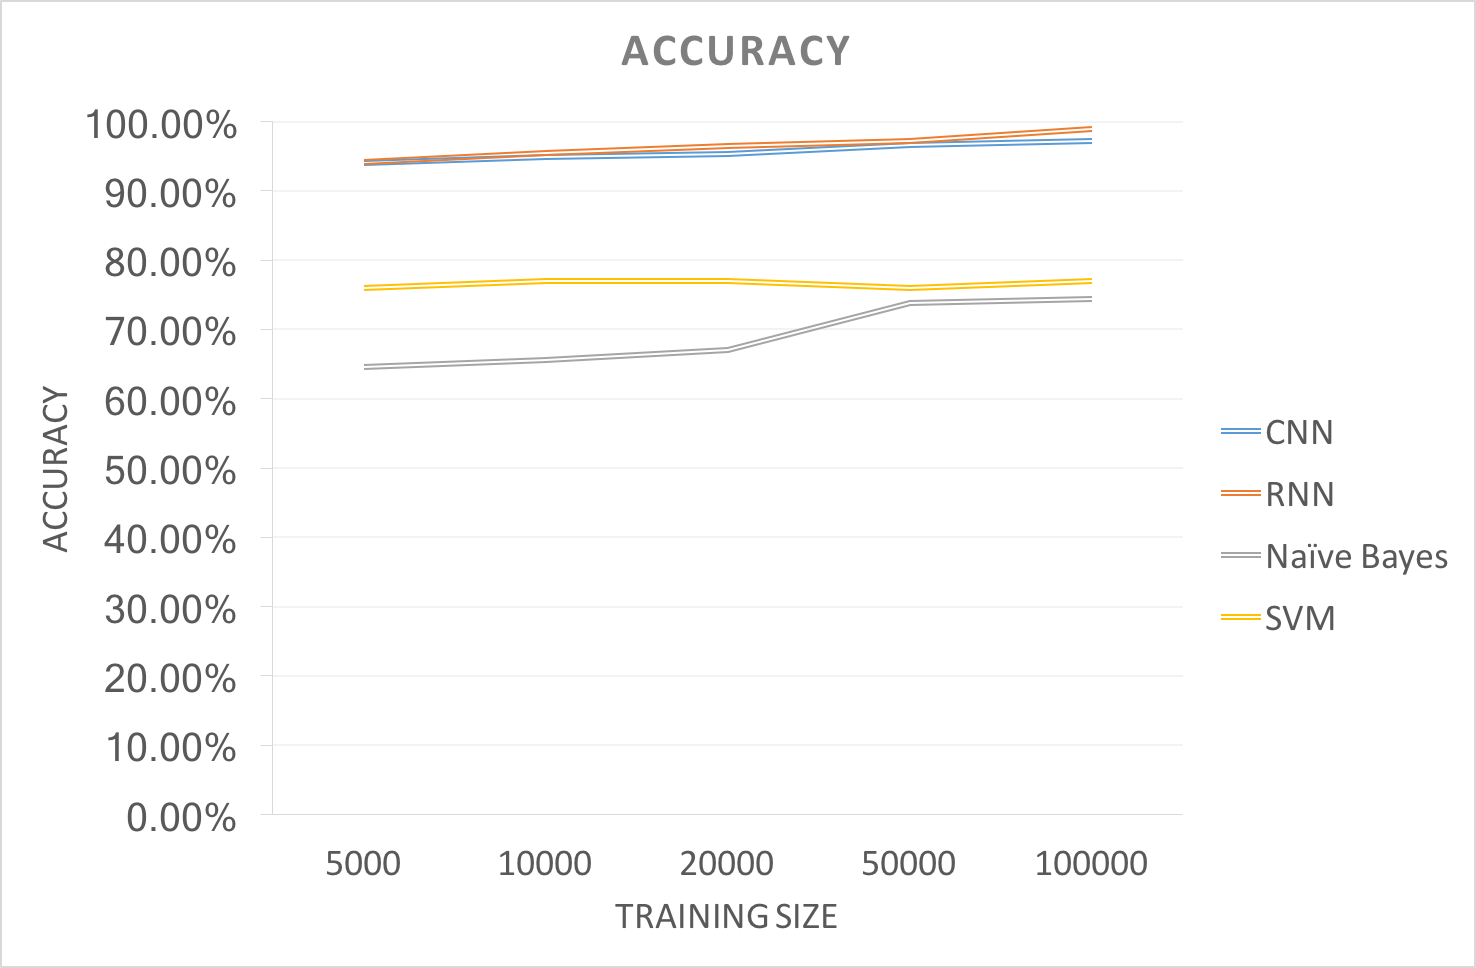
\includegraphics[width=0.9\linewidth]{accuracy1}
	\caption{Model performance with different sizes of training data.}
	\label{fig:acc1}
\end{figure} 
 \begin{figure}[htb]
	\centering
	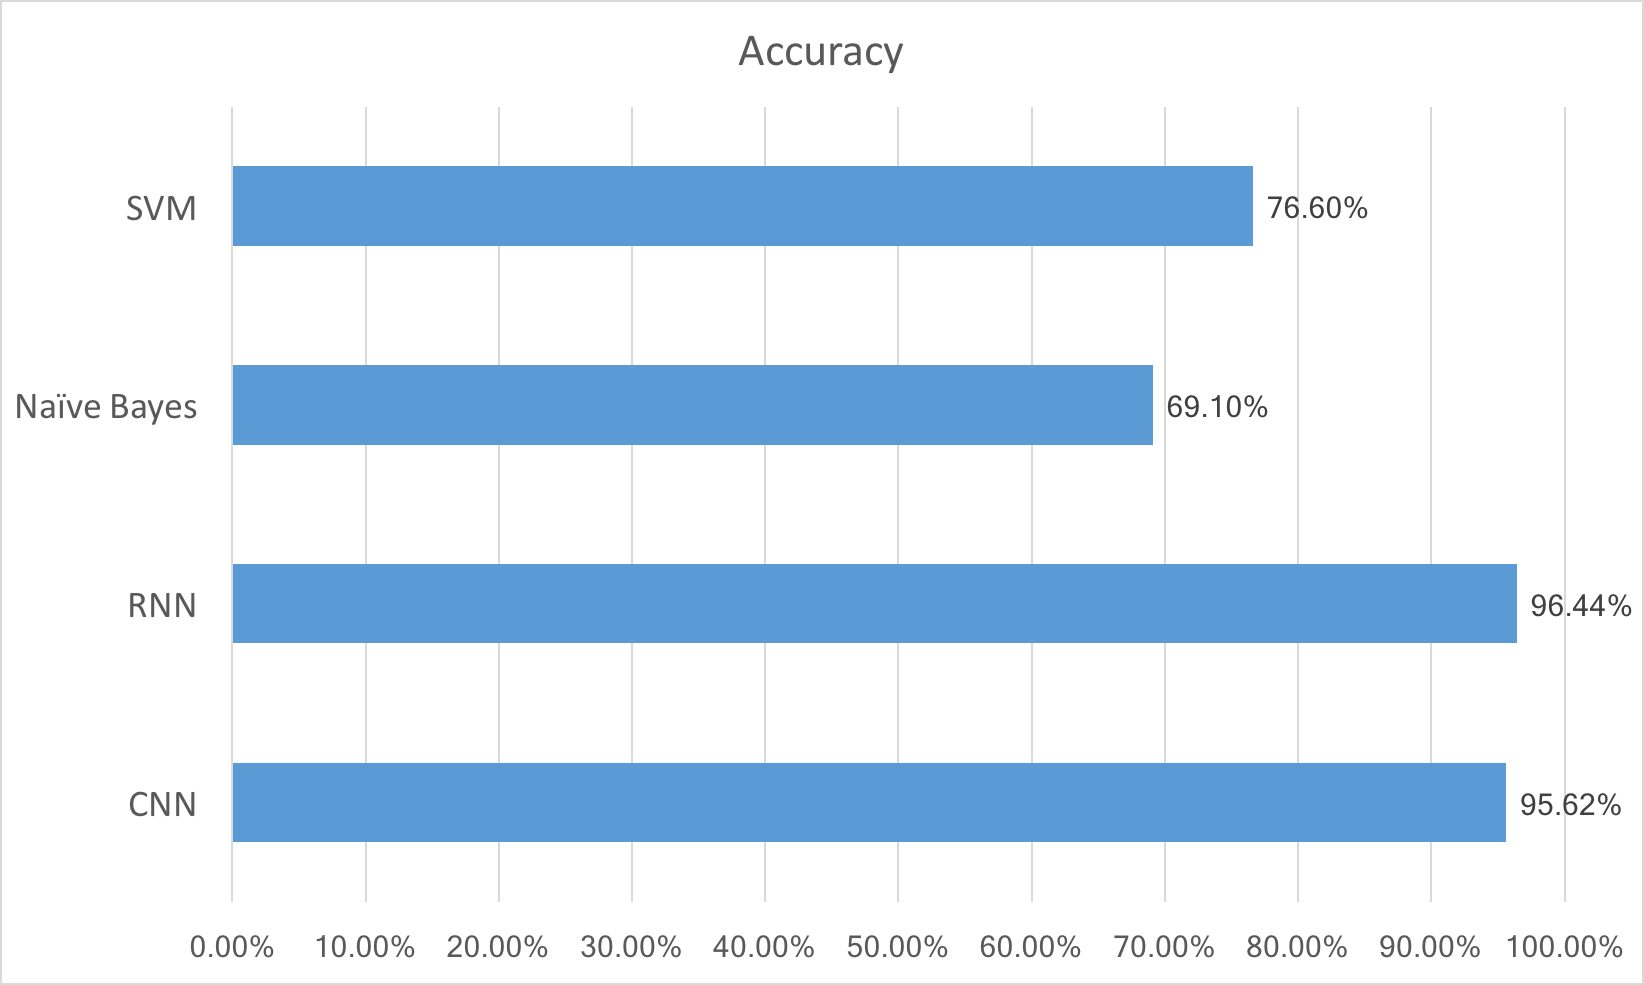
\includegraphics[width=0.9\linewidth]{accuracy2}
	\caption{Average performance}
	\label{fig:acc2}
\end{figure} 

\subsubsection{Comparison with CNN model}
RNN model outperform CNN in terms of accuracy and convergence rate. 
%
We can see from Figure \ref{fig:acc1} that RNN accuracy is larger than CNN.
%
Moreover,  Figure \ref{fig:acc3} shows the accuracy results of training data when in different epoch times. For each epoch (iteration), we feed the RNN and CNN model with a batch of 64 tweets which are mapped to vector representations.
%
We can see that in ,the training accuracy of RNN becomes stable after 12 iterations. But for CNN, it takes more iterations to achieve robustness (after 26 iteration).
% 

 \begin{figure}[htb]
	\centering
	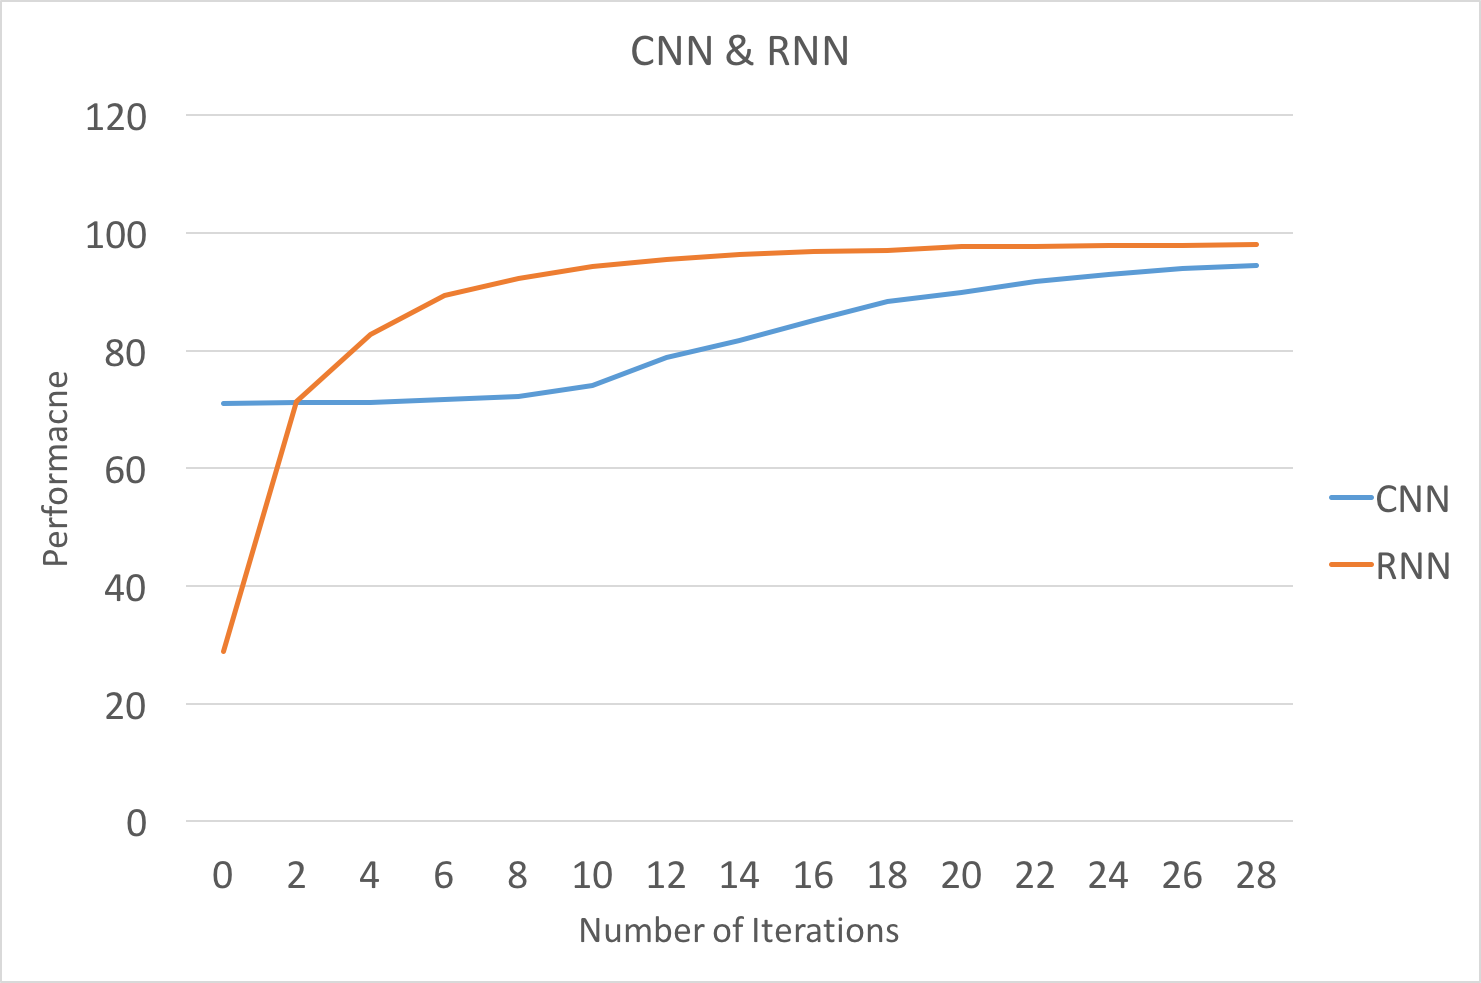
\includegraphics[width=0.9\linewidth]{accuracy3}
	\caption{Convergence rate of RNN and CNN.}
	\label{fig:acc3}
\end{figure} 


 


% !TEX root = /Users/zhuzhuangdi/Desktop/MSUCourses/NaturalLanguageProcessing842/CSE842/FinalReport/latex/final.tex

\section{Conclusion and Future Work}  
%
In this project, we implement an RNN model to achieve tweet sentiment classification using word-to-vector features.
%
We also implement three baseline models to compare with our approach.
%
We use a SVM model and Naive Bayes model to compare our results with traditional bag-of-words classifiers, and use a standard Convolution Neural Network model to compare with deep learning classifiers.
%
Our approach outperforms all these baseline models in terms of accuracy and convergence rate.

In the future, we plan to explore with more complex neural network models.
%
Especially, RNNs has various structures and we may benefit from advanced RNN models. For example, Matrix Vector RNN \cite{socher2013recursive} and Recursive Neural Tensor Network \cite{socher2012semantic} already prove it can efficiently classify among movie reviews. 
%
These models may further improve the results of tweets sentiment classification.
%
We also plan to explore how twitter features, such as emotions, hashtags and short hands, can be used to improve the performance of prediction on the sentiment label of tweets.

% More neural network-based sentiment analysis models have been proposed recently.
%Socher \etal created a recursive model to build the sentiment label of a sentence through its parse tree \cite{socher2012semantic}. Each constituent in the sentence is associated with a vector-matrix representation.The vector conveys the meaning of the constituent, while the matrix conveys how it changes the meaning of neighboring constituents.

 
}
 

\bibliographystyle{abbrv}
\bibliography{proposal} 
 

\end{document}
